% Chapter 33: Treating Light as Rays
\chapter{Treating Light as Rays}

\step{A Counterintuitive Opening}

Try something now: put a chopstick into a glass half full of clear water and look from the side. The chopstick ``breaks'' at the surface: its submerged section looks bent and displaced to one side. Pull it out and it is perfectly intact; put it back and it ``breaks'' again.

Of course you do not really believe that water magically bends chopsticks. But here is the problem: your eyes have always trusted that ``what you see lies in the direction you look.'' This time they confidently point in the wrong direction. Light from the submerged chopstick has clearly reached your eyes, yet your eyes ``place'' it somewhere wrong. Something must have happened to the light on its journey from water into air.

This ``deception'' is more than a dinner-table trick; it has affected practical skills. Among people who spear fish along rivers and coasts, a rule has passed down the generations: aim below the fish you see, not directly at it. A child's first attempts usually miss because the spear targets the position reported by the eyes, where the fish simply is not. Experienced fishers may never discuss physics, but they have already paid tuition to the deceptive water surface.

% BEGIN TRANSLATOR SAFETY NOTE
\textbf{Translator safety note:} Do not dive or extend a breath-hold simply to reproduce this view. Never breath-hold dive alone or hyperventilate beforehand; obtain suitable training and supervision. See \href{https://world.dan.org/alert-diver/article/freediving-safety-awareness/}{Divers Alert Network breath-hold safety guidance}.
% END TRANSLATOR SAFETY NOTE

Something stranger happens below the surface. Dive to the bottom of a swimming pool and look up. If you are deep enough and look at a sufficiently oblique angle, the surface above is not a transparent window but a mirror: reflections of poolside lights and the ceiling appear clearly, while the scenery outside the water completely disappears. The same surface is a window from above and a mirror from below. When does a window become a mirror? What is the criterion?

Here is another inexpensive but endlessly intriguing sight. Summer sunlight heats an asphalt road until it is scorching. Looking ahead while driving, you see apparent puddles reflecting the sky and oncoming headlights. Approach them and they vanish, while new puddles appear farther away. Drivers know they are false, yet they look remarkably like reflections from water. The ``lakes'' seen by desert travelers are the same phenomenon. There is no water surface, yet light seems to have reflected from a nonexistent mirror.

\begin{mainline}
All this chapter's difficulties boil down to one question: light travels in straight lines, as shadows and pinhole cameras demonstrate, but suddenly bends when it crosses the boundary between two materials, and the amount of bending follows a precise rule. What is that rule, and what deeper principle does it obey?
\end{mainline}

\step{Make a Guess First}

Before turning the page, write down your guess: what most likely makes the chopstick appear ``broken'' at the surface?

First guess: an illusion in the eyes or brain. Water itself does nothing to light; the brain is simply unused to seeing through water and invents the wrong picture.

Second guess: water acts like ``resistance,'' dragging light down to a lower speed. Light struggles to travel and veers aside, like someone stumbling while wading.

Third guess: light changes direction at the boundary between two materials according to a definite rule. The deflection is neither an illusion nor vague ``resistance,'' but a measurable angular change that repeats consistently.

Also predict something we will check later: if light enters water obliquely from air, will it turn toward the vertical or away from it? What happens in the reverse direction, from water into air? Write down your answers.

One more subtle question: does some obliquely incident light enter the water while some reflects from the surface, or can only one of those things happen? If you are unsure, visit a lake: at dusk, you can see both the reflected sky and stones underwater. Both coexist. This fact will help us eliminate some models shortly.

\step{Hands-on Experiment}

\begin{experiment}[The Disappearing Coin]
Find an opaque bowl or mug and put a coin on its bottom. Stand in position, then slowly step backward, or move the bowl forward, until its rim just hides the coin. Keep your head and the bowl still.

Now ask someone to pour water slowly into the bowl while you maintain your position and watch its bottom. As the water rises, the hidden coin gradually ``floats'' back into view until you can see it completely. If the liquid poured is another transparent liquid, such as cooking oil, the extent of this apparent rise differs.
\end{experiment}

The coin has not moved, your eyes have not moved, and the bowl has not moved. The only change is the added water. The conclusion is unavoidable: at the surface, water bends the light traveling from the coin to your eyes. Moreover, the coin emerges from behind the rim, showing that the bending has a definite direction rather than happening randomly.

% BEGIN TRANSLATOR SAFETY NOTE
\textbf{Translator safety note:} Keep laser beams and their reflections away from eyes, people, and animals; do not use a laser pointer as a toy or raise the apparatus into anyone's eye line. See \href{https://www.fda.gov/consumers/consumer-updates/laser-toys-how-keep-kids-safe}{FDA laser safety guidance}.
% END TRANSLATOR SAFETY NOTE

If you have a laser pointer, you can make another set of observations. Remember never to aim it directly at eyes. Fill a transparent rectangular container with water and mix in one or two drops of milk to reveal the light's path. Shine the laser obliquely onto the surface from the air. You will see three things at once: one beam bounces back into the air (reflection); another enters the water but bends noticeably at the surface (refraction); and the refracted beam lies closer to the vertical than the incident beam. Replace the water with sugar solution or oil and the amount of bending changes.

Answer three observational questions: as the incident beam becomes more oblique, does the refracted beam depart more or less from the original direction? Does light bend when it enters perpendicular to the surface? Raise the container and direct the laser upward through the water toward the surface, increasing its inclination: what happens? Remember the third observation; it will star in the chapter's second half.

\step{The Old Model Runs into Trouble}

First, a word in the old model's defense. ``Light travels in straight lines'' is an enormously successful empirical rule. It explains hand shadows: the hand blocks the light, leaving darkness behind where light cannot reach. It explains solar eclipses: the Moon sits directly between Sun and Earth, and observers in its umbra see the Sun completely covered. It explains pinhole cameras: light from each object point passes through the pinhole to a definite point on the screen, producing an inverted image. Craftspeople use it to align straight edges, surveyors to sight targets, and ancient observers used an upright stick's solar shadow to determine seasonal markers. In this language, light is something flying straight, and all of optics amounts to drawing straight lines.

But at a water surface, this language immediately hits a wall.

The first wall is refraction. ``Light travels straight'' provides no role for a ``boundary.'' The deflections in the chopstick and coin experiments are definite and repeatable, not vague edge effects. The old model can say ``light bent,'' but not by how much, in which direction, or why glass bends it more than water.

The second wall is that it cannot even explain its specialty, reflection. Everyone knows ``the angle of incidence equals the angle of reflection,'' but why? ``Traveling straight'' describes a route without giving any reason those angles must be equal. It is like recording a thousand vehicles' paths through an intersection without understanding why every driver turns that way: data, but no explanation.

The third and subtlest wall is that the model cannot say clearly whether ``light travels straight'' is an experimental fact or a modeling assumption. Strictly, it is a conditional approximation: light does travel straight in a uniform material, but a change of material, such as air to water, or a nonuniform material, such as air above a sun-heated road, breaks that straightness. Treating a conditional approximation as an unconditional law is precisely the mistake for which intuition will later pay tuition.

\begin{mainline}
The old model's accounts amount to this: it accurately \textbf{describes} three things, straight-line propagation, reflection, and refraction, but \textbf{explains} none. We need a new conceptual tool that encompasses all three descriptions and answers ``why this particular angle?''
\end{mainline}

\step{Inventing New Concepts}

Begin with an abstraction that is enormously important and easily misunderstood: the \textbf{light ray}.

Draw a thin arrowed line on paper to represent light's direction and route. That line is a ray. \textbf{What it resembles}: a hiker's route marked on a map, showing the starting point, direction, and turns. \textbf{What it does not resemble}: a physically existing filament. The bright line you see from a laser pointer appears because dust and moisture along its path scatter a small fraction of its light into your eyes. Light traveling through a vacuum is completely invisible from the side. Nor is a ray ``light's physical substance''; you cannot cut it or weigh it. It is simply a geometrical name for light's direction of travel. The abstraction is powerful because shadows, reflection, and refraction all become geometrical problems about ``lines,'' which can be drawn, measured, and calculated.

Now translate the three phenomena into geometry. At the boundary, draw a reference line perpendicular to the surface: the \textbf{normal}. The angle between the incident ray and normal is the \textbf{angle of incidence}; between the reflected ray and normal, the \textbf{angle of reflection}; and between the ray entering the other material and normal, the \textbf{angle of refraction}. All three angles are measured from the normal, not the surface. This convention makes the laws as simple as possible.

\begin{center}
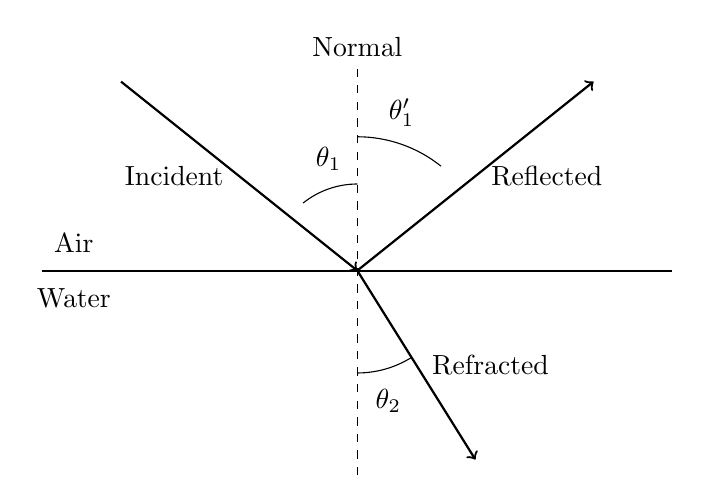
\begin{tikzpicture}[scale=1.0]
  % Interface and normal
  \draw[thick] (-4,0) -- (4,0);
  \draw[dashed] (0,-2.6) -- (0,2.6) node[above] {Normal};
  \node at (-3.6,0.35) {Air};
  \node at (-3.6,-0.35) {Water};
  % Incident ray
  \draw[->,thick] (-3,2.4) -- (0,0) node[midway,left=2pt] {Incident};
  % Reflected ray
  \draw[->,thick] (0,0) -- (3,2.4) node[midway,right=2pt] {Reflected};
  % Refracted ray (toward normal)
  \draw[->,thick] (0,0) -- (1.5,-2.4) node[midway,right=2pt] {Refracted};
  % Angle labels
  \draw (0,1.1) arc (90:128.7:1.1) node[pos=0.5,above=3pt] {$\theta_1$};
  \draw (0,1.7) arc (90:51.3:1.7) node[pos=0.5,above=3pt] {$\theta_1'$};
  \draw (0,-1.3) arc (270:302:1.3) node[pos=0.55,below=4pt] {$\theta_2$};
\end{tikzpicture}
\end{center}

Next come two experimental facts distilled from extensive measurements:

\textbf{The law of reflection}: the reflected ray lies in the plane defined by the incident ray and normal, and the angle of reflection equals the angle of incidence, \(\theta_1'=\theta_1\). The same law applies to mirrors, water surfaces, floors, and any smooth interface, with enough precision for satellite ranging. Its everyday appearances are surprisingly numerous: periscopes use two parallel mirrors to turn light twice, allowing people in trenches or underwater to see past obstacles. Roadside reflectors and the ``cat's eyes'' in bicycle rear reflectors contain many tiny right-angle reflecting structures that return headlight beams almost along their original paths to drivers' eyes. Returning light toward its source makes them especially bright at night.

\textbf{The law of refraction}: the refracted ray also lies in that plane, but its angle generally differs from the incident angle. For a given incident angle, the bending from air into water is fixed, while that into glass has another fixed value. Each transparent material therefore carries its own number describing its ``bending ability.'' We call it the \textbf{refractive index}, denoted \(n\). The index of vacuum, approximately also air, is defined as \(1\); water is about \(1.33\), ordinary glass about \(1.5\), and diamond as high as \(2.42\). The larger the refractive index, the more strongly the boundary bends light.

Refractive index also has a deeper physical identity. We can directly measure light's speed in different materials: in vacuum, \(c\approx 3.0\times10^8\) meters per second; in water, only about \(2.25\times10^8\) meters per second; and in glass, about \(2.0\times10^8\) meters per second. Measurements show that for every transparent material,
\[
v=\frac{c}{n},\qquad\text{or}\qquad n=\frac{c}{v}.
\]
Refractive index is the ratio of light's speed in vacuum to its speed in the medium. Pause over this equation: a geometrical number describing ``how much light bends'' is also the number describing ``how slowly light travels in this material.'' Bending and slowing are two aspects of the same thing. For this chapter, we accept that experimental fact. Why matter determines both will become clear only after Chapters 35 and 36 treat light as a wave and examine its interaction with matter.

So far, reflection and refraction remain separate empirical rules. Could they share a root? In the seventeenth century, Fermat proposed an idea almost bizarre in its boldness: \textbf{between two points, light always follows a path whose travel time is stationary, usually the shortest.}

Do not dismiss this as mysterious yet. Imagine a lifeguard on a beach with a drowning swimmer diagonally offshore. The lifeguard runs quickly on sand but swims slowly in water. Should the rescue follow a straight line? No. The sensible route runs farther along the beach toward an entry point farther upshore, minimizing the ``slow water journey.'' The fastest route is not straight but bends at the shoreline, and the larger the speed difference, the sharper the bend. This is exactly light's behavior at water: it moves quickly on the ``beach'' of air and ``swims slowly'' in water, taking a route that bends toward the normal at the boundary.

\textbf{Where the analogy fits}: two speeds, two regions, and an optimum crossing point have exactly the same structure as refraction. \textbf{Where it does not}: the lifeguard is conscious, compares options, and decides; light does not. ``Light chooses the quickest path'' does not mean it tests every route before setting off and then selects one. This is the language of a mathematical model, not light's inner monologue. Why a physical law with no sense of time appears in ``least-time'' form will begin to emerge in Chapter 35's wave picture: Fermat's principle is a natural consequence of waves with extremely short wavelengths.

Fermat's principle brings another gift: \textbf{reversibility of light paths}. If ``least time'' is a property of the path from \(A\) to \(B\), then sending light back from \(B\) along that same path still gives the quickest route. If you can see a diver's eyes from above the water, the diver can also see you. Mutual visibility never requires either person to ``emit a line of sight''; only actual light travels. Reversibility may sound trivial, but it is the key to halving many calculations when designing complex optical instruments later.

Let us also redraw shadows, since they will shortly testify in the section on limits. A point source, such as a laser illuminating a tiny hole, produces sharp shadow edges. Extended sources such as the Sun or a fluorescent tube produce two regions: the umbra, where light from every direction is blocked, and the penumbra, where only some is blocked. In a solar eclipse, the Moon projects these shadows onto Earth: observers in the umbra see a total eclipse, while those in the penumbra see a partial one. Everything can be drawn using straight-line propagation alone, one of the ray model's finest victories. Remember its condition: the source and obstacles must be much larger than light's wavelength.

\step{The Model in One Sentence}

\begin{oneline}
Model light as traveling along ``rays'': it travels straight through a uniform material; at a boundary, some bounces back with equal incident and reflected angles, while some refracts according to Snell's law. Both rules rest on a deeper principle: light follows a path of stationary travel time (Fermat's principle), and the refractive index \(n=c/v\) records how much each material slows it.
\end{oneline}

Distinguish three levels in that sentence: experimental facts (straight-line propagation, reflection, refraction, and light's speed in media); mathematical models (rays, angles, refractive index, and optical path length); and explanatory frameworks (Fermat's principle). Mixing facts, models, and explanations causes most confused ideas in optics.

\step{The Mathematical Translator}

Now turn intuition into calculable equations.

The equation for \textbf{reflection} is almost too simple to look like a formula:
\[
\theta_1'=\theta_1 .
\]
Check special cases. Normal incidence: \(\theta_1=0\) gives \(\theta_1'=0\), so light retraces its path. Shine a flashlight perpendicular to a mirror and its spot returns toward your hand: correct. Grazing incidence: as \(\theta_1\to 90^\circ\), reflected light also leaves almost along the surface. A skipping stone bounces ``perfectly'' from water at very low angles, and low sunset light reflects strongly from water: correct. Reverse the direction: light sent backward along the reflected path emerges along the original incident path. Reversibility: correct.

The equation for \textbf{refraction} is Snell's law:
\[
n_1\sin\theta_1=n_2\sin\theta_2 .
\]
Read both sides: the left contains the incident-side material and angle; the right, those on the refracted side. The combination \(n\sin\theta\) stays unchanged across the boundary. A ``slower'' material, with larger \(n\), requires a smaller angle to compensate: light lies closer to the normal in the slower material.

Check special cases one by one.

Check one: normal incidence. With \(\theta_1=0\), the left side vanishes, so \(\theta_2=0\): perpendicular entry causes no deflection. This matches the laser experiment. But beware a subtle trap: unchanged direction does not mean nothing changed. The speed changes from \(c\) to \(c/n\), so traversing the same thickness takes longer. Your eyes respond only to direction, so you cannot see that change, but light has already ``entered it in the accounts.''

Check two: identical materials. If \(n_1=n_2\), then \(\theta_2=\theta_1\): no deflection, naturally, since there is no real boundary. An elegant application is a glass rod immersed in oil with almost the same refractive index: the rod becomes ``invisible.'' Without bending at the interface, light passes straight through and the eyes cannot locate the glass.

Check three: air into water. With \(n_1=1\) and \(n_2=1.33\), we have \(\sin\theta_2=\sin\theta_1/1.33\). Take \(\theta_1=45^\circ\): \(\sin\theta_2\approx 0.707/1.33\approx 0.53\), giving \(\theta_2\approx 32^\circ\). The refracted ray is noticeably closer to the normal, matching the experiment. Did you guess correctly?

Check four: water into air, with a steadily increasing incident angle. Here \(n_1=1.33\) and \(n_2=1\), requiring \(\sin\theta_2=1.33\sin\theta_1\). But sine cannot exceed \(1\). When \(\theta_1\) grows until \(1.33\sin\theta_1=1\), the refracted angle reaches \(90^\circ\). Increase the incident angle further and the equation has \textbf{no solution}. Mathematics sounds an alarm: the refracted ray disappears. The critical angle satisfies
\[
\sin\theta_c=\frac{n_2}{n_1}\quad(n_1>n_2).
\]
For water to air, \(\sin\theta_c=1/1.33\), giving \(\theta_c\approx 48.6^\circ\). Beyond that angle, all light reflects at the boundary without a trace escaping: \textbf{total internal reflection}. Here is an intuition-defying counterexample. Most people expect ``some light always gets through a boundary; only the amount varies,'' since glass both reflects and transmits. Total internal reflection says otherwise: beyond the critical angle, transmission does not merely decrease; it vanishes, and reflectivity jumps to a perfect hundred percent, more complete than any mirror, which still absorbs a few percent.

Total internal reflection is the lifeblood of optical fibers. A glass thread not much thicker than a hair has a core with a slightly higher refractive index than its cladding. Light traveling sufficiently obliquely in the core reflects totally at each wall encounter, zigzagging through a mirrored tunnel without leaking out for kilometers or tens of kilometers. Submarine fiber cables carry an entire film's signal from one continent to another this way. Medical endoscopes and gastroscopes likewise use bundles of fibers to deliver light into the body and carry images out.

\begin{center}
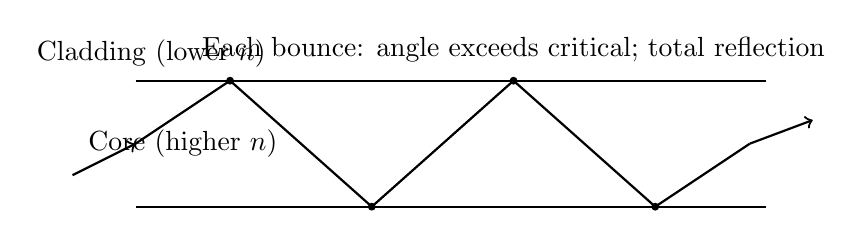
\begin{tikzpicture}[scale=1.0]
  % Optical fiber
  \draw[thick] (0,0.8) -- (8,0.8);
  \draw[thick] (0,-0.8) -- (8,-0.8);
  \node at (0.2,1.15) {Cladding (lower $n$)};
  \node at (0.6,0) {Core (higher $n$)};
  % Zigzag ray
  \draw[->,thick] (-0.8,-0.4) -- (0,0) ;
  \draw[thick] (0,0) -- (1.2,0.8) -- (3.0,-0.8) -- (4.8,0.8) -- (6.6,-0.8) -- (7.8,0);
  \draw[->,thick] (7.8,0) -- (8.6,0.3);
  % Reflection points
  \foreach \x/\y in {1.2/0.8, 3.0/-0.8, 4.8/0.8, 6.6/-0.8}
    \fill (\x,\y) circle (0.05);
  \node at (4.8,1.2) {Each bounce: angle exceeds critical; total reflection};
\end{tikzpicture}
\end{center}

We can also calculate \textbf{apparent depth}. Looking vertically down from above the surface, an object at underwater depth \(h\) appears at depth
\[
h'=\frac{h}{n}.
\]
Use real numbers: for a pool \(2.0\) meters deep and \(n=1.33\), we find \(h'\approx 2.0/1.33\approx 1.5\) meters. The eyes report a depth one-quarter shallower than reality. That is why a child jumping into apparently ``waist-deep'' water can end up submerged, and it quantifies the fishing rule ``aim below the fish.'' This estimate assumes a nearly vertical line of sight; the derivation appears in the mathematical bridge below.

\begin{mathbridge}
\textbf{Deriving Snell's law from Fermat's principle.} Let light travel from point \(A\) in air, through point \(P\) on the interface, to point \(B\) in water. Let the perpendicular distances from \(A\) and \(B\) to the interface be \(a\) and \(b\); their perpendicular feet are separated by a fixed distance \(L\). Let the distance from \(P\) to the foot below \(A\) be \(x\). The total time is
\[
T(x)=\frac{n_1}{c}\sqrt{a^2+x^2}+\frac{n_2}{c}\sqrt{b^2+(L-x)^2}\,.
\]
Fermat's principle says the actual \(x\) makes \(T\) stationary, so \(\mathrm{d}T/\mathrm{d}x=0\):
\[
n_1\frac{x}{\sqrt{a^2+x^2}}=n_2\frac{L-x}{\sqrt{b^2+(L-x)^2}}\,.
\]
The left side is exactly \(n_1\sin\theta_1\), and the right exactly \(n_2\sin\theta_2\). Snell's law emerges complete, signs and all, from the single requirement of stationary travel time.

\textbf{Deriving apparent depth.} Take two closely spaced rays from a submerged object: one travels vertically upward, the other at a small angle \(\theta_2\) to the normal. Snell's law changes the latter's angle on emergence to \(\theta_1\approx n\,\theta_2\), using the small-angle approximation. The eye extends the emerging rays backward in straight lines; they meet at depth \(h'=h\tan\theta_2/\tan\theta_1\approx h/n\). The small-angle approximation matters: oblique viewing requires a correction to apparent depth, which is why a pool bottom looks distorted from the side.
\end{mathbridge}

\begin{challenge}
\textbf{``Shortest'' should really be ``stationary.''} Fermat's principle precisely says that optical path length, travel time multiplied by \(c\), or \(\int n\,\mathrm{d}s\), is \textbf{stationary}: it may be a minimum, maximum, or saddle-like turning point. An ellipsoidal mirror offers a clean counterexample. Light from focus \(F_1\) reflects to focus \(F_2\), and all paths have exactly equal optical lengths: an ellipse is defined by a constant sum of distances. Every path is stationary; none is ``shortest.'' With more general interface shapes, a stationary path can even maximize optical length. The popular phrase ``principle of least time'' happens to work in most everyday situations, but is wrong as a universal law. Stationarity is what Fermat's principle really requires.

\textbf{A hidden passage to mechanics.} Readers of Chapters 13 and 14 may recognize the flavor: in mechanics, a particle follows a trajectory of stationary action; in optics, light follows a path of stationary optical length. This is no coincidence. Hamilton first recognized the shared mathematical structure of mechanics and geometrical optics: particle trajectories play the same role in mechanics as rays in optics. This connection later helped guide Schrödinger toward wave mechanics; Chapter 43 reaches its other end.
\end{challenge}

\step{The Model's Limits}

The ray model is an excellent map, but uncharted features can trip you on the actual journey.

\textbf{Limit one: obstacles must not be too small.} The ray model assumes strictly straight propagation and perfectly sharp shadow edges. Yet inspect a pencil's shadow under a fluorescent tube: its edge is not knife-sharp but grades from light to dark. Pass light through a sufficiently narrow slit and it spreads instead of continuing straight. These phenomena necessarily appear when obstacle sizes become comparable to light's wavelength, roughly a few hundred nanometers, less than a hundredth of a hair's thickness. The ray model has nothing to say: it is not giving a wrong answer but facing a question it was never built to answer. Why light bends around obstacles and spreads more through narrower slits is Chapter 35's main course in wave optics. There we will see that rays are not wrong; they are the limiting picture as wavelength tends to zero.

\textbf{Limit two: rays are not objects, and do not explain ``how much.''} This chapter's laws govern direction, not energy distribution. Why is water's reflection bright at oblique angles but the surface almost transparent viewed head-on? How do reflected and refracted fractions vary with angle and polarization? These require Chapter 36's Fresnel equations. Discussing ``intensity'' with rays alone is like measuring altitude on a map that does not show it.

\textbf{Limit three: refractive index depends on color.} Saying ``water's index is \(1.33\)'' actually gives its value for yellow-green light; violet light has a slightly higher index in water than red light. This is why a prism separates white light into a colored band and why diamond fire is multicolored. The ray model can accommodate ``a different \(n\) for each color,'' but cannot explain why \(n\) changes. That requires the interaction between light and charges inside matter, also reserved for Chapters 35 and 36.

\textbf{Limit four: common misuses.} First, treating ``light travels straight'' as an unconditional cosmic law: it holds only in uniform media, with mirages as counterexamples, discussed below. Second, imagining light slowing in matter because ``photons ricochet between atoms and take detours.'' That is not the correct microscopic picture. The incident electromagnetic field drives charges in matter to oscillate; those charges reradiate, and the combined wave propagates at phase velocity \(c/n\), as Chapter 36 details. Third, treating Fermat's principle as evidence that ``light thinks.'' It is an extraordinarily effective calculation rule whose deeper explanation lies in waves, not purpose or intention.

Finally, connect rays with earlier knowledge. Chapter 25 described light as an electromagnetic wave, electric and magnetic fields propagating through space. This chapter draws thin lines instead. How can both descriptions coexist? The ray model is a sketch of electromagnetic waves when their wavelength is much smaller than every obstacle. When everything is enormous from the wavelength's perspective, wave behavior reduces to geometrical lines, just as a meandering river reduces to a curve on a large-scale map. This chapter does not overturn ``light is an electromagnetic wave''; it finds the most convenient way to use that fact. The model fails precisely where wave details begin to show.

\step{Explaining the Opening Phenomenon}

Now settle the opening's four outstanding accounts.

\textbf{Why the chopstick ``breaks.''} Light from each submerged point bends away from the normal on leaving the water, according to Snell's law: from water to air, \(n\) decreases and the angle increases. Your eyes and brain do one thing: extend the received light backward in straight lines. Those extensions converge at positions shallower and closer to you than the actual chopstick, so the underwater section appears raised and displaced, producing a bend at the surface. This is not an optical illusion but the eyes faithfully applying ``light travels straight,'' a rule that happens to work above the surface and fail below it. Your eyes have not been deceived; they simply do not know that part of the route passed through water.

\textbf{When water changes from window to mirror.} For a diver looking up, the angle between sightline and surface determines the incident angle. Below the critical angle of \(48.6^\circ\), the surface is a window onto the world above. Beyond it, total internal reflection turns the surface into a perfect mirror of underwater scenery. A circular bright opening, Snell's window, therefore appears overhead: the entire above-water hemisphere is compressed into that circle, while outside it lies a mirrored underwater world.

\textbf{The road's ``puddles.''} In fierce sunshine, the road heats the air a few centimeters above it. Hot air is less dense and has a slightly lower refractive index than the cooler air above, creating a graded medium whose index increases continuously upward. Light descending obliquely from the sky bends farther from the normal as it crosses each ``faster'' layer. Its path curves continuously until it passes the local critical condition, turns upward, and enters the driver's eyes. The driver extends the light backward along a straight line and ``sees'' the reflected sky on the road. The brain insists there is water because it recognizes only mirror reflection as a way for the sky to appear on a road. There is no water; an entire graded air layer impersonates a mirror. This is an inferior mirage. Superior mirages above cold layers over seas or polar regions, with objects apparently suspended in the air, follow the same principle with the temperature gradient reversed. Mirages are also everyday instances of nature openly departing from the approximation ``light travels straight in a uniform medium.'' They happen daily; most people mistake the evidence for illusion.

\textbf{The Sun ``lifted'' by the atmosphere.} Graded-index tricks occur daily at the horizon, on a smaller scale. Atmospheric refractive index rises continuously from \(1\) in space to about \(1.0003\) at sea level. Starlight and sunlight arriving near the horizon bend incrementally downward through it. Consequently, when the Sun's lower edge appears just to touch the horizon, its true position is already entirely below it: atmospheric refraction has lifted it by about half a degree, roughly one solar diameter. The time equivalent is tangible: Earth takes about two minutes to turn through half a degree, so the atmosphere ``steals'' about two extra minutes of daylight for us each morning and evening. Astronomical sunrise and sunset tables must include this refraction correction to match the clock. This is graded refraction's quietest and most widespread performance: no desert or heatwave required, just a planet wrapped in air.

\begin{center}
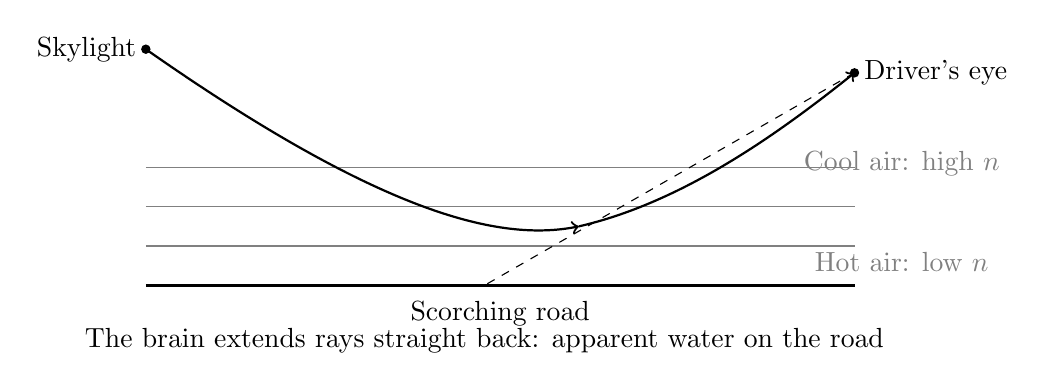
\begin{tikzpicture}[scale=1.0]
  % Graded air layers
  \foreach \y in {0.5,1.0,1.5}
    \draw[thin,gray] (0,\y) -- (9,\y);
  \draw[thick] (0,0) -- (9,0) node[midway,below=2pt] {Scorching road};
  \node[gray] at (9.6,1.55) {Cool air: high $n$};
  \node[gray] at (9.6,0.3) {Hot air: low $n$};
  % Curved ray
  \draw[thick,->] (0,3.0) .. controls (3,0.9) and (4.5,0.55) .. (5.5,0.75);
  \draw[thick,->] (5.5,0.75) .. controls (6.8,1.05) and (8,1.9) .. (9,2.7);
  \fill (0,3.0) circle (0.06) node[left] {Skylight};
  \fill (9,2.7) circle (0.06) node[right] {Driver's eye};
  % Virtual image
  \draw[dashed] (9,2.7) -- (4.3,0) ;
  \node at (4.3,-0.7) {The brain extends rays straight back: apparent water on the road};
\end{tikzpicture}
\end{center}

\textbf{The laser pointer's beam.} And the incidental question: why can you see the beam? Dust in the air scatters a little light in every direction, some into your eyes. In a truly clean vacuum, a beam passing before you would be invisible. Seeing the beam is evidence precisely that light has ``not'' traveled entirely straight into your eyes.

\step{Thought Experiments and Challenges}

\begin{thought}[Send Light Around the Earth]
Light travels straight and Earth is round, so a beam sent along the horizon disappears for good. But graded refractive index offers a wild possibility: suppose an atmosphere encircled the whole planet with its index decreasing smoothly with altitude at exactly the right rate. Could a beam curve continuously downward along an arc parallel to Earth's surface, circle the globe, and return to the back of your head?

In theory, this works if the refractive-index gradient meets the precise condition, roughly that the light path's curvature equals Earth's surface curvature. Atmospheric ``waveguiding'' really has been used in radar and beyond-horizon communication, although typically it extends range by only a few hundred kilometers, not a complete circuit. The practical obstacles are that Earth's atmosphere is only a few tens of kilometers thick and its gradient far too weak; it is also nonuniform and turbulent, unable to maintain so delicate a path. The thought experiment's value is this: in the ray model, once \(n\) may vary continuously, straight lines lose their privilege. Rays can bend into any shape, depending on the refractive-index distribution. Keep this key for later: when gravity curves spacetime itself, light's bending will return in another guise in Chapter 41.
\end{thought}

\begin{puzzles}
\item A diver looking up sees a circular bright window containing the entire above-water world: sky, Sun, and shoreline trees. Outside is a mirror image of underwater scenery. Use the critical angle to explain why scenery from every above-water direction, a whole hemisphere, fits into a cone with half-angle only \(48.6^\circ\). (Hint: light arriving from near the above-water horizon has an incident angle near \(90^\circ\). What is its largest possible refracted angle? Where does Snell's law impose a ceiling? It is angles, not the number of objects, that are compressed.)
\item Diamond has refractive index \(2.42\), ordinary glass about \(1.5\). Why does a well-cut diamond sparkle so much more than glass, with light reluctant to leave once inside? (Hint: calculate each material's critical angle to air. A smaller critical angle traps what range of incident angles by total internal reflection? A diamond's dozens of facets design an inescapable mirror maze for light.)
\item An optical fiber is \(1\) kilometer long, and light travels through its glass core at \(2.0\times10^8\) meters per second. How long does a straight axial trip take? If total internal reflection makes the path zigzag and \(20\%\) longer than the axis, how long does it take? What trouble does this time difference cause for signals that should arrive together? (Hint: calculate the straight-path time, of order microseconds, then multiply by \(1.2\). Different arrival times blur successive high-speed pulses together, which is why engineers restrict ray angles inside fibers.)
\item Fermat says light follows a stationary-time path. But how does light ``know'' at departure which route is quickest? Does it first try every route? Answer using this chapter's framework: which parts of that statement are legitimate model language, and which mistake the model for fact? Which chapter's picture holds the real answer? (Hint: distinguish ``the stationary form of a law'' from ``a particle making decisions.'' In Chapter 35, waves traverse all paths simultaneously, with mutual reinforcement only near stationary paths. Then ``comparing every route'' gains a non-anthropomorphic explanation.)
\end{puzzles}

\begin{mainline}
We have done three things: abstracted light into rays and used two geometrical laws, reflection and refraction, to unify shadows, mirrors, and bending at water surfaces; joined ``bending'' and ``slowing'' through refractive index \(n=c/v\); and gathered both laws into Fermat's statement that light follows stationary-time paths. Next chapter adds mirrors and lenses to this geometrical language to explain image formation in eyes, cameras, and telescopes. The following chapter will send light through two slits and force us to replace the ray map: light's other face is a wave.
\end{mainline}
